%! Author = joels
%! Date = 13/07/2021

\section{Introduction}
\subsection{Browser-based Applications}
\textcolor{b}{\textbf{Benefits:}}
\begin{itemize}[topsep=0pt, leftmargin=3mm]
    \setlength\itemsep{-0.3em}
    \item Work from anywhere, anytime
    \item Platform independent, including mobile
    \item No software update, no application, easy maintenance
    \item Software can be provided as a service (SaaS - pay as you go)
    \item Code separation
\end{itemize}
\textcolor{b}{\textbf{Liabilities:}}
\begin{itemize}[topsep=0pt, leftmargin=3mm]
    \setlength\itemsep{-0.3em}
    \item No data sovereignty (Datenhoheit)
    \item Limited/restricted hardware access
    \item SEO - Search engines must execute JavaScript
    \item More complex deployment strategies
\end{itemize}
\subsection{SPA}
In an SPA, either all necessary code is retrieved with a single page load or the appropriate resources are dynamically loaded and added to the page as necessary. Uses AJAX and HTML5\\
\textcolor{b}{\textbf{Traditional Architecture:}} Server renders a new HTML page with every call. (Major logic on server, no architectural separation between presentation and logic)\\
\textcolor{b}{\textbf{SPA Architecture:}} Website interacts with user by rewriting parts of the DOM (moves logic from server to client, server provides APIs like REST/GraphQL) $\rightarrow$ After first load, all interaction with the Server happens through AJAX
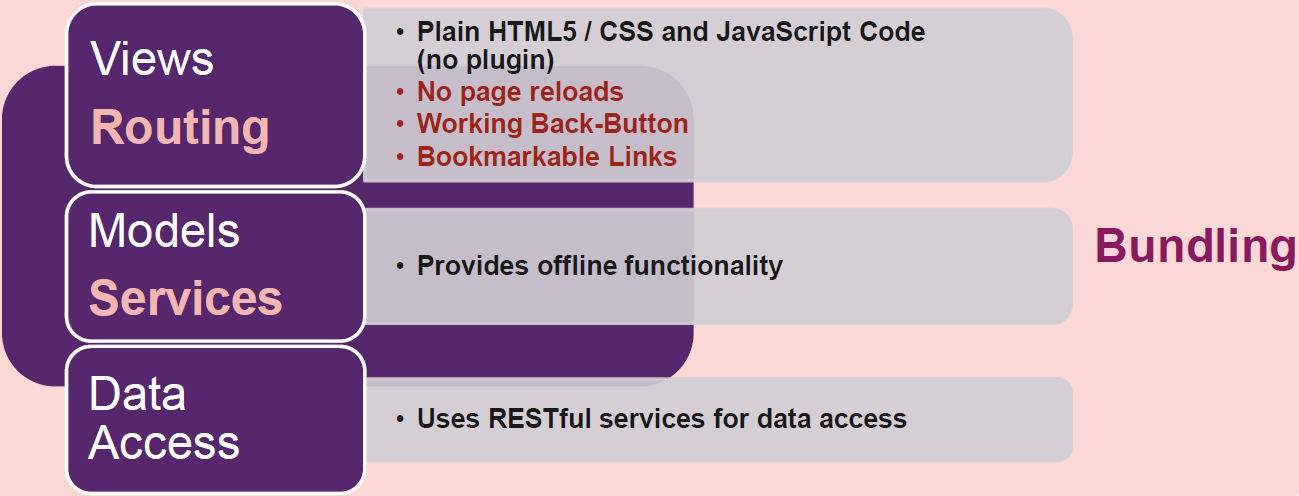
\includegraphics[width=0.8\linewidth]{spa_overview.png}\\
\textcolor{b}{\textbf{SPA aus Kundensicht:}} Sobald Desktop ähnliche User Experience gewünscht ist. Mehr möglichkeit für komplexe WebApps mit viel Animationen/graphischen Elementen.\\
\textcolor{b}{\textbf{Technischer Nutzen von SPA:}} Server App wird von Darstellung getrennt: Separation of Concerns, Bessere Wartbarkeit das Client-Codes, Aufteilung in Teams/Kompetenzzentren\\
\textcolor{b}{\textbf{Bundling SPAs:}} E.g. WebPack
\begin{itemize}[topsep=0pt, leftmargin=3mm]
    \setlength\itemsep{-0.3em}
    \item All JS code must be delivered over potentially slow networks
    \item Bundling and minifying the source leads to smaller footprint
    \item Larger SPAs need a reliable dependency management
    \item Initial footprint can be reduced by loading dependent modules on-demand
\end{itemize}
\textcolor{b}{\textbf{Dependency Injection Benefits:}}
\begin{itemize}[topsep=0pt, leftmargin=3mm]
    \setlength\itemsep{-0.3em}
    \item Reduces coupling between consumer and the implementation
    \item The contracts between the classes are based on interfaces
    \item Classes relate to each other not directly, but mediated by thier interfaces
    \item Supports the open/closed principle
    \item Allows flexible replacement of an implementation
\end{itemize}